%%%%%%%%%%%%%%%%%%%%%%%%%%%%%%%%%%%%%%%%%%%%%%%
%%% Template for lab reports used at STIMA
%%%%%%%%%%%%%%%%%%%%%%%%%%%%%%%%%%%%%%%%%%%%%%%

%%%%%%%%%%%%%%%%%%%%%%%%%%%%%% Sets the document class for the document
% Openany is added to remove the book style of starting every new chapter on an odd page (not needed for reports)
\documentclass[12pt,english, openany]{book}

%%%%%%%%%%%%%%%%%%%%%%%%%%%%%% Loading packages that alter the style
\usepackage{caption}
\usepackage{subfigure}
\usepackage[]{graphicx}
\usepackage[]{color}
\usepackage{alltt}
\usepackage[T1]{fontenc}
\usepackage[utf8]{inputenc}
\setcounter{secnumdepth}{3}
\setcounter{tocdepth}{3}
\setlength{\parskip}{\smallskipamount}
\setlength{\parindent}{0pt}

% Set page margins
\usepackage[top=66pt,bottom=66pt,left=66pt,right=66pt]{geometry}

% Package used for placeholder text
\usepackage{lipsum}

% Prevents LaTeX from filling out a page to the bottom
\raggedbottom

% Adding both languages
\usepackage[english, italian]{babel}

% All page numbers positioned at the bottom of the page
\usepackage{fancyhdr}
\fancyhf{} % clear all header and footers
\fancyfoot[C]{\thepage}
\renewcommand{\headrulewidth}{0pt} % remove the header rule
\pagestyle{fancy}

% Changes the style of chapter headings
\usepackage{titlesec}
\titleformat{\chapter}
   {\normalfont\LARGE\bfseries}{\thechapter.}{1em}{}
% Change distance between chapter header and text
\titlespacing{\chapter}{0pt}{50pt}{2\baselineskip}

% Adds table captions above the table per default
\usepackage{float}
\floatstyle{plaintop}
\restylefloat{table}

% Adds space between caption and table
\usepackage[tableposition=top]{caption}
\usepackage{listings}
\usepackage{xcolor}

\lstset{basicstyle=\small,
        % numbers=left, 
        % numberstyle=\tiny, 
        keywordstyle=\color{blue},
        breaklines=true,
        % commentstyle=\color[cmyk]{1,0,1,0}, 
        frame=single, 
        % extendedchars=false, 
        %xleftmargin=2em,xrightmargin=2em, aboveskip=1em, 
        % tabsize=4, 
        showspaces=false,
}


% Adds hyperlinks to references and ToC
\usepackage{hyperref}
\hypersetup{hidelinks,linkcolor = black} % Changes the link color to black and hides the hideous red border that usually is created

% If multiple images are to be added, a folder (path) with all the images can be added here 
\graphicspath{ {Figures/} }

% Separates the first part of the report/thesis in Roman numerals
\frontmatter


%%%%%%%%%%%%%%%%%%%%%%%%%%%%%% Starts the document
\begin{document}

%%% Selects the language to be used for the first couple of pages
\selectlanguage{english}

%%%%% Adds the title page
\begin{titlepage}
	\clearpage\thispagestyle{empty}
	\centering
	\vspace{1cm}

	% Titles
	% Information about the University
	{\normalsize NYU – TANDON SCHOOL OF ENGINEERING \\ 
		CS-GY 6083 - B, SPRING 2020 \\
		Principles of Database Systems \par}
		\vspace{3cm}
	{\Huge \textbf{PROJECT PART I}} \\
	\vspace{1cm}
	\begin{table}[H]
	\centering
    \begin{tabular}{cccc}
    Qianyong & Tang & N11366182 & qt344 \\
    Tianyu   & Gu   & N13364566 & tg1899     
    \end{tabular}
    \end{table}
	\vspace{6cm}
    
    \centering 
\includegraphics[scale=0.8]{Tandon-Engineering.png}
    
    \vspace{0.5cm}
		
	% Set the date
	{\normalsize \today \par}
	
	\pagebreak

\end{titlepage}

% Adds a table of contents
\tableofcontents{}

%%%%%%%%%%%%%%%%%%%%%%%%%%%%%%%%%%%%%%%%%%%%%%%%%%%%%%%%%%%%%%%%%%%%%%%%%%%%%%%%%%%%%%%%%%%%
%%%%%%%%%%%%%%%%%%%%%%%%%%%%%%%%%%%%%%%%%%%%%%%%%%%%%%%%%%%%%%%%%%%%%%%%%%%%%%%%%%%%%%%%%%%%
%%%%% Text body starts here!
\mainmatter

\chapter{Description}
This report describes the database design created for the company We Do Secure (WDS), used to help WDS deal with recently expanded operation on offering Auto and Home insurance to their customers. The database provides the function to store information required by WDS of customer, policy, home, auto, auto driver, customer payment and invoice. Moreover, the database design indicates the relationship between these entities clearly. The detailed design and assumptions are explained in the following pages. The robustness of the database is proved by generating sample data and several practice SQL queries with flexibility. Our model can hold complex situations such as multiple homes and autos for one customer. All the previous records of a customer are stored. Our model also supports multiple drivers for multiple autos. There are more features for our model. For further information, the corresponding codes and results are shown in next sections.


\chapter{Assumptions}
\begin{enumerate}
    \item A customer has only two subtypes, auto-customer(acustomer) and home-customer (hcustomer).
    \item A customer has to be either acustomer or hcustomer, or both.
    \item An hcustomer can have multiple homes, and each home can have multiple home insurance policies.
    \item An acustomer can have multiple autos, and each auto can have multiple auto insurance policies.
    \item An auto may can have multiple drivers and a driver can drive multiple cars.
    \item A driver is distinct from a customer in the database.
    \item An hpolicy for a home can have multiple payments, i.e., installments.
    \item An apolicy for an auto can have multiple payments, i.e., installments.
    \item An hpolicy for a home only generate one invoice.
    \item An apolicy for an auto only generate one invoice.
    \item Multiple payments for a certain hpolicy for a home correspond to one invoice.
    \item Multiple payments for a certain apolicy for an auto correspond to one invoice.
    \item Each payment corresponds to either home policy or auto policy but cannot be both.
    \item A policy has only two subtypes, auto-policy(apolicy) and home-policy(hpolicy).
    \item A policy has to be either apolicy or hpolicy, but cannot be both.
\end{enumerate}

\chapter{Results}

\section{Problem A}
    \begin{figure}[H]
        \centering
        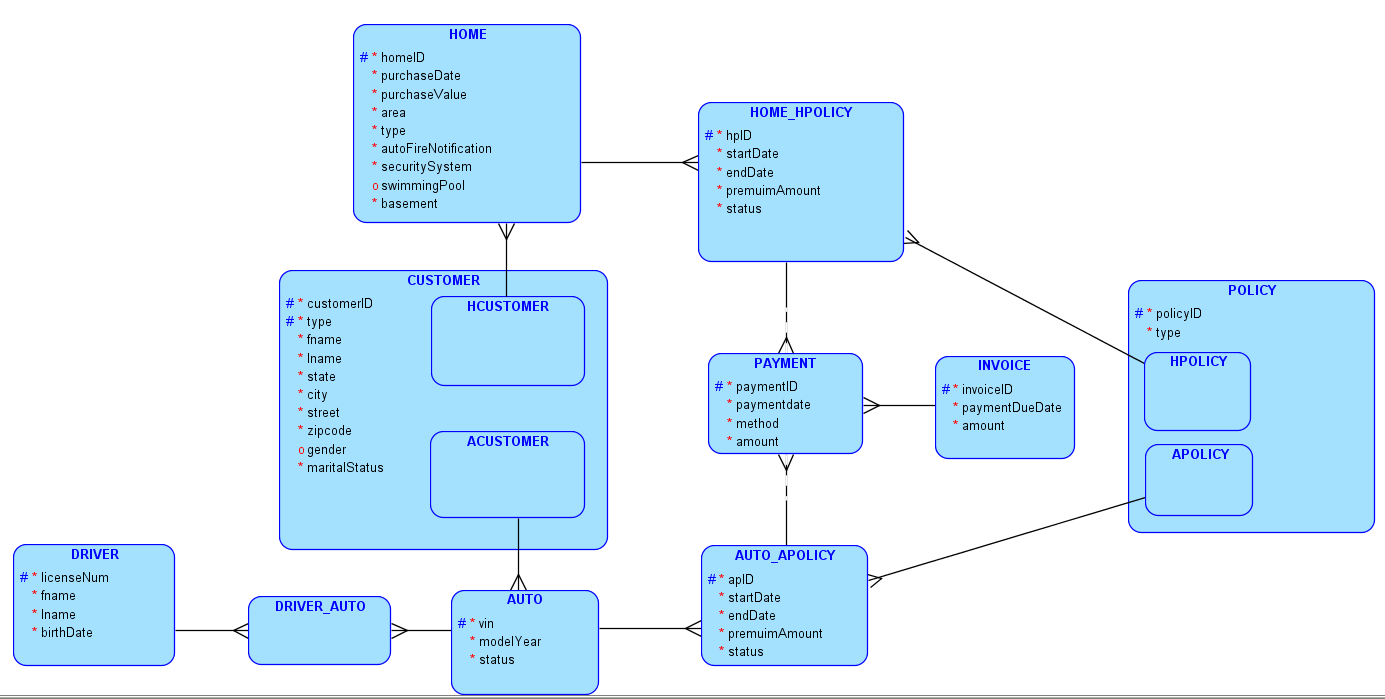
\includegraphics[scale=0.35]{logical.png}
    \end{figure}
    
\section{Problem B}
    \begin{figure}[H]
        \centering
        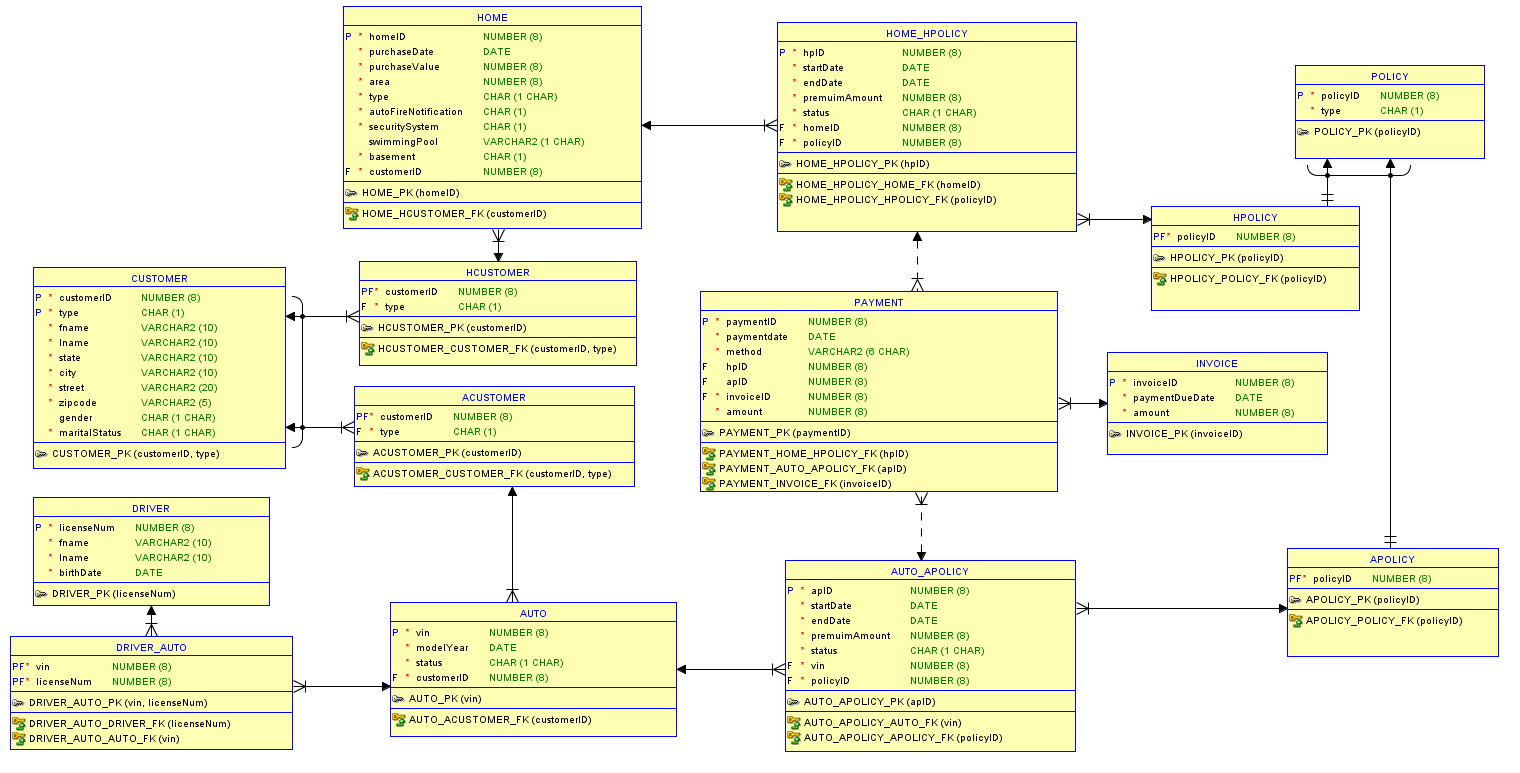
\includegraphics[scale=0.33]{relational.png}
    \end{figure}
    
\section{Problem C}
\lstinputlisting {scripts/c_WDS.sql}
\section{Problem D}
\lstinputlisting {scripts/d_constraints.sql}
\section{Problem E}
\lstinputlisting {scripts/e_sample.sql}
\section{Problem F}
\lstinputlisting [language=SQL]{scripts/f_list.sql}

\begin{figure}[H]
        \centering
        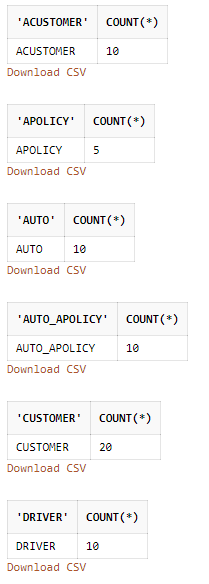
\includegraphics[scale=0.5]{f1.png}
\end{figure}
\begin{figure}[H]
        \centering
        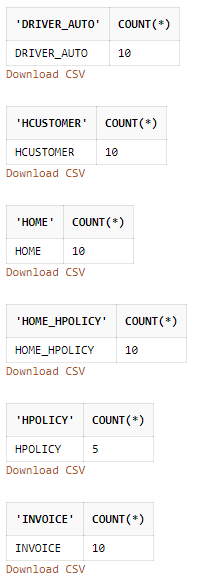
\includegraphics[scale=0.5]{f2.png}
\end{figure}
\begin{figure}[H]
        \centering
        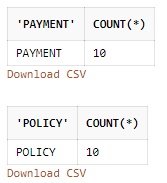
\includegraphics[scale=0.5]{f3.png}
\end{figure}
\section{Problem G}
\lstinputlisting [language=SQL]{scripts/g_detail.sql}
\begin{figure}[H]
        \centering
        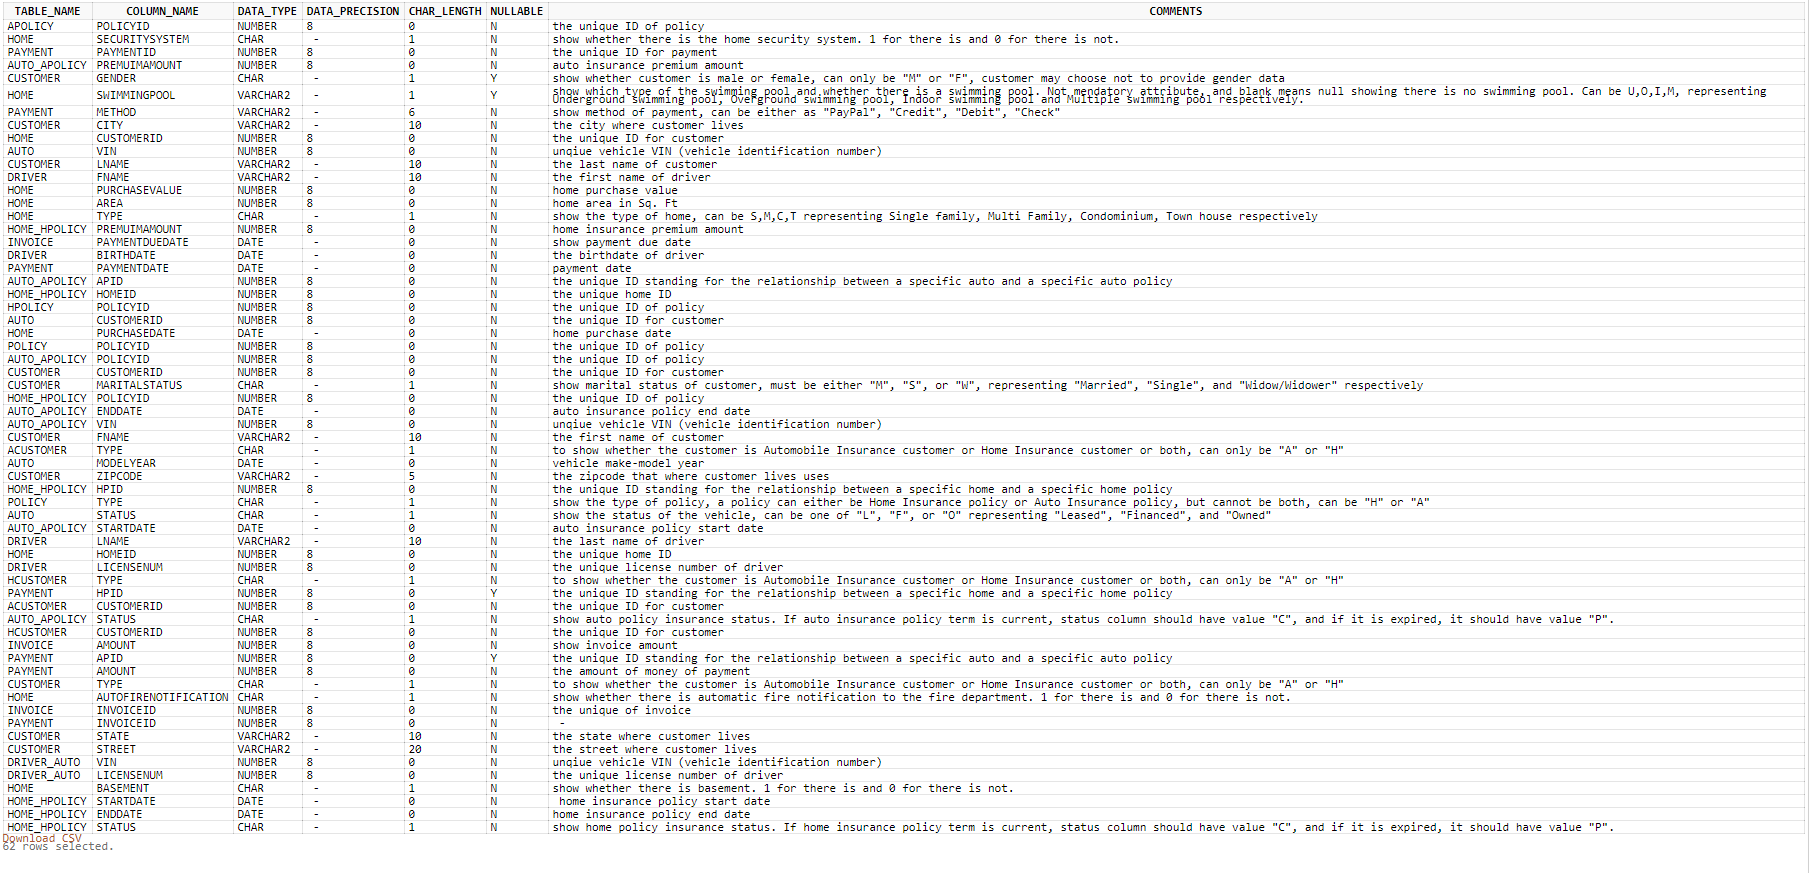
\includegraphics[scale=0.27]{g1.png}
\end{figure}
\begin{figure}[H]
        \centering
        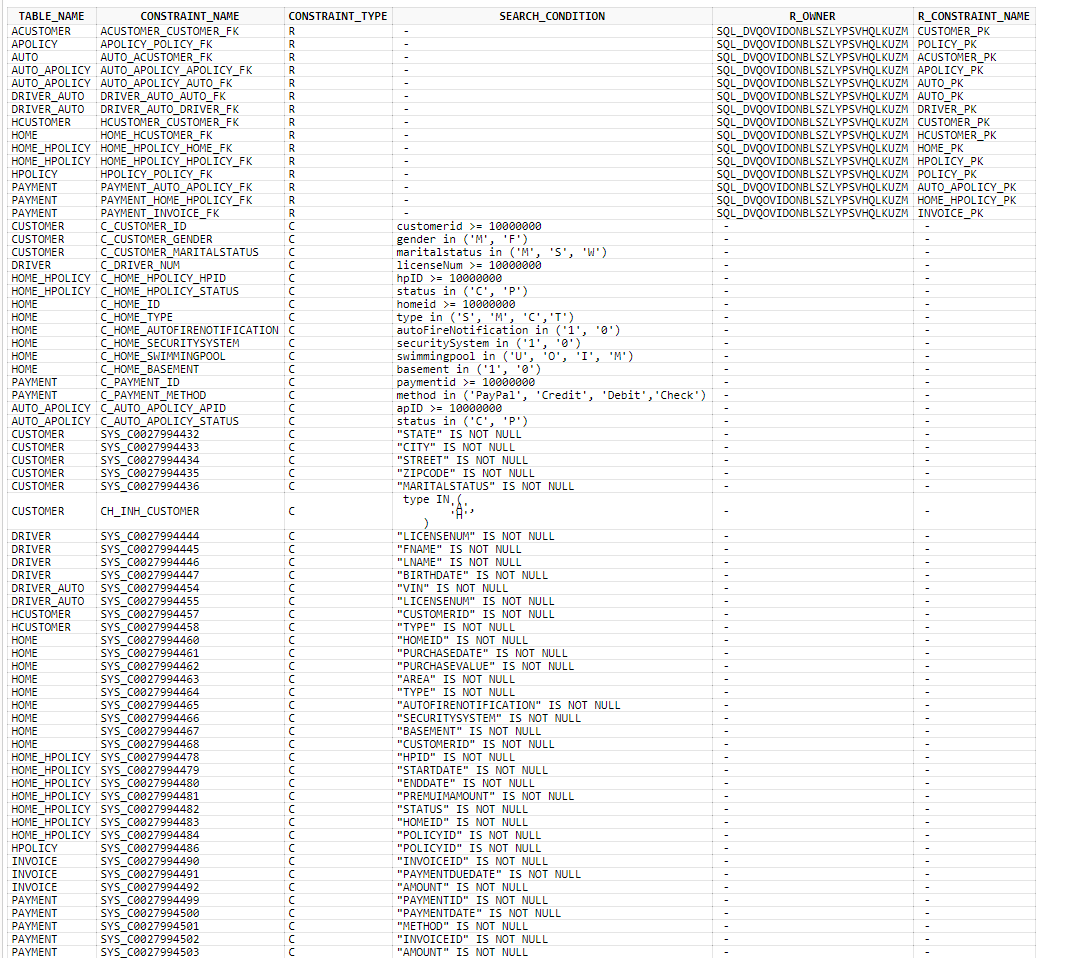
\includegraphics[scale=0.45]{g2_1.png}
\end{figure}
\begin{figure}[H]
        \centering
        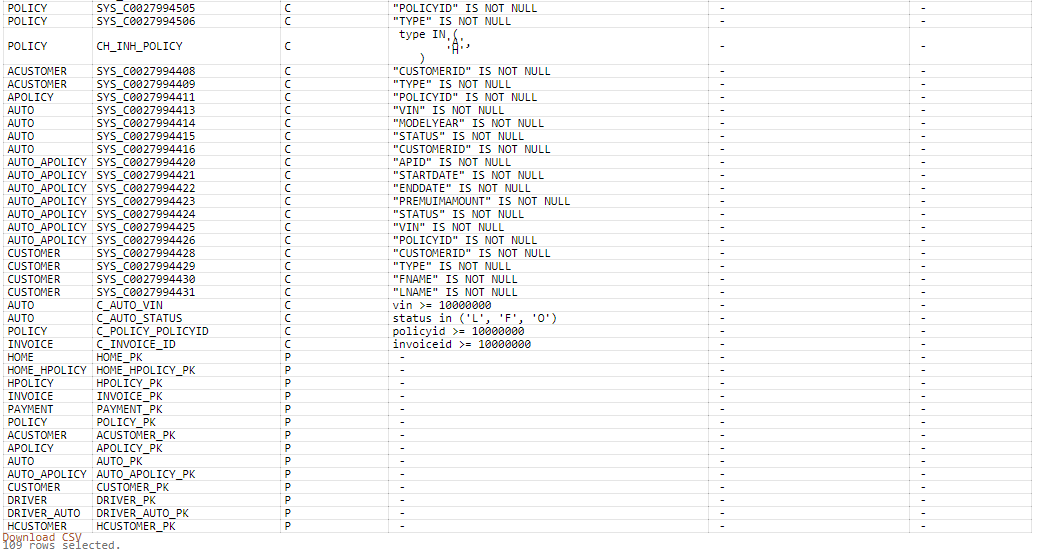
\includegraphics[scale=0.45]{g2_2.png}
\end{figure}
\section{Problem H}
\subsection{Q1: Table joins with at least 3 tables in join}
Select query: 
\begin{lstlisting}[language=SQL]
    SELECT A.vin, C.lname
    FROM AUTO A INNER JOIN DRIVER_AUTO B ON
    A.vin = B.vin
    INNER JOIN DRIVER C ON
    B.licenseNum = C.licenseNum
\end{lstlisting}

Result of the query:
    \begin{figure}[H]
        \centering
        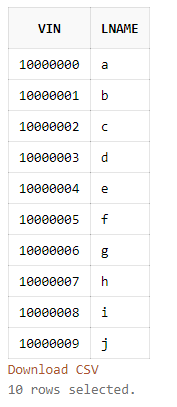
\includegraphics[scale=0.6]{h1.png}
    \end{figure}
    
Purpose of query: select the vin of the car and its corresponding drivers' last name.

\subsection{Q2: Multi-row subquery}
Select query: 
\begin{lstlisting}[language=SQL]
    SELECT homeID, purchasedate, purchasevalue, area 
    FROM home 
    WHERE homeID IN
    (
    SELECT homeID 
    FROM home_hpolicy 
    WHERE status = 'C'
    );
\end{lstlisting}

Result of the query:
    \begin{figure}[H]
        \centering
        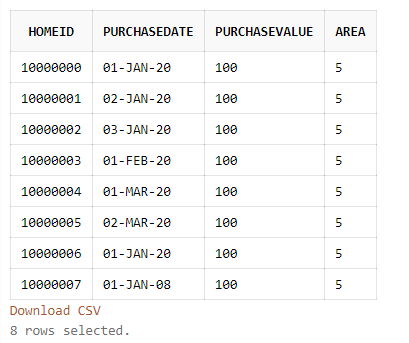
\includegraphics[scale=0.6]{h2.png}
    \end{figure}
    
Purpose of query: select homeID, purchasedate, purchasevalue and area of home whose home policy status is "Current".

\subsection{Q3: Co-related subquery}
Select query: 
\begin{lstlisting}[language=SQL]
    SELECT *
    FROM payment pa
    WHERE amount> 
    (
    SELECT AVG(amount)
    FROM payment
    WHERE method = pa.method
    );
\end{lstlisting}

Result of the query:
    \begin{figure}[H]
        \centering
        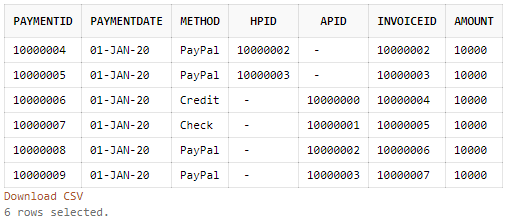
\includegraphics[scale=0.6]{h3.png}
    \end{figure}
    
Purpose of query: select the information of payment whose amount is larger than the average amount of the payment with the same payment method.

\subsection{Q4: SET operator query}
Select query: 
\begin{lstlisting}[language=SQL]
    SELECT policyID 
    FROM HPOLICY
    INTERSECT
    SELECT policyID
    FROM HOME_HPOLICY;
\end{lstlisting}

Result of the query:
    \begin{figure}[H]
        \centering
        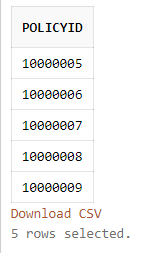
\includegraphics[scale=0.6]{h4.png}
    \end{figure}
    
Purpose of query: select the home policy ID that the policy is chosen and being used by home customer.

\subsection{Q5: Query with any analytical function or in line view or WITH clause}
Select query: 
\begin{lstlisting}[language=SQL]
    SELECT
     *
    FROM
    (
        SELECT
            homeid,
            purchasedate,
            purchasevalue
        FROM
            home
        ORDER BY
            purchasedate DESC
    )
    WHERE
    ROWNUM <= 10;
\end{lstlisting}

Result of the query:
    \begin{figure}[H]
        \centering
        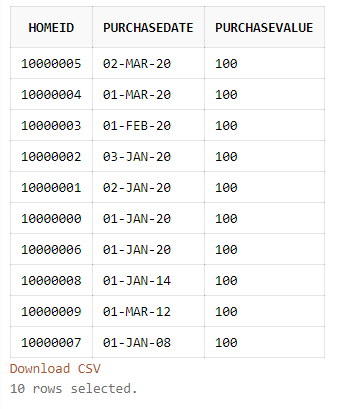
\includegraphics[scale=0.6]{h5.png}
    \end{figure}
    
Purpose of query: select no more than 10 rows of homeID, purchaseDate and purchseValue from home with the descendent ordering of purchase value.



\end{document}
